\chapter{Data Characteristics}
A critical criterion for assessing the validity of a developed model or diagnostic algorithm is its performance on real-world data, whether sourced from controlled experiments or operational vehicles. For this study, Cummins supplied both test-cell and truck data. Test-cell data were obtained by operating the test cell using established standard drive cycles. Truck data were collected from four long-haul trucks over a one-day period, first with fresh (degreened) catalysts and later after catalyst aging.
%===============================================================================
Test-cell data were collected for both aged and degreened catalysts under three established drive cycles:
\begin{enumerate}
        \item Hot Federal Test Procedure (hFTP)
        \item Cold Federal Test Procedure (cFTP)
        \item Ramped Mode Cycle (RMC)
\end{enumerate}
The main distinction among these three cycles is the operating temperature during the drive cycles (Figure~\ref{fig::test_cell_temp_profiles}). The RMC test operates at higher temperatures than the FTP tests. Although hFTP and cFTP have overlapping temperature ranges, cFTP starts at a much lower temperature. Table~\ref{tab::test_cell_data_vars} summarizes the variables included in the test-cell data.
%==
\begin{figure}[!ht]
        \centering
        \includegraphics[width=0.7\textwidth]{./figs/2-data/test_cell_temp_range.png}
        \caption{Drive Cycle Temperature Profiles of Test Cell Data}
        \label{fig::test_cell_temp_profiles}
\end{figure}
%==
\begin{table}[!ht]
\centering
\caption{Test Cell Data Variables}
\label{tab::test_cell_data_vars}
\begin{tabular}{l l l l}
   \hline \hline
   Data Name &
   Units &
   Variable &
   Description \\ \hline \hline
   %==========================================================================
   LOG\_TM &
   sec &
   $t$ &
   Time
   \\
   %==========================================================================
   EXHAUST\_FLOW &
   kg/min &
   $F$ &
   Exhaust Flow Rate
   \\
   %==========================================================================
   V\_AIM\_TRC\_DPF\_OOUT &
   $\lx{^o}{C}$ &
   $T_{in}$ &
   DPF-out (SCR-in) Gas Temperature
   \\
   % =========================================================================
   V\_AIM\_TRC\_SCR\_OUT &
   $\lx{^o}{C}$ &
   $T_{out}$ &
   SCR/ASC out Gas Temperature
   \\
   % ==========================================================================
   V\_UIM\_FLM\_ESTUREAINJRATE &
   ml/s &
   $u_{inj}$ &
   DEF (Urea Sol.) Dosing Rate
   \\
   % ==========================================================================
   ENG\_CW\_NOX\_FTIR\_COR\_U2 &
   ppm &
   $\con{NO_x}^{out}$ &
   Engine-Out $NO_x$
   \\
   % ==========================================================================
   EXH\_CW\_NOX\_COR\_U1 &
   ppm &
   $\con{NO_x}^{in}$ &
   Tailpipe $NO_x$
   \\
   % ==========================================================================
   EXH\_CW\_AMMONIA\_MEA &
   ppm &
   $\con{NH_3}^{out}$ &
   Tailpipe $NH_3$
   \\
   % ==========================================================================
   EONOX\_COMP\_VALUE &
   ppm &
   $\con{NO_x}^{in}$ &
   Engine-out $NO_x$
   \\
   % ==========================================================================
   V\_SCM\_PPM\_SCR\_OUT\_NOX &
   ppm &
   $\con{NO_x}^{out}_{\chi}$ &
   SCR-out $NO_x$ (cross-sensitive)
   \\
   \hline \hline
\end{tabular}
\end{table}
% =====
A key advantage of test-cell data is the inclusion of FTIR (Fourier Transform Infrared Spectroscopy) sensor measurements, which can estimate both NOx and NH3 gas concentrations. In contrast, the commercial NOx sensor is cross-sensitive to ammonia, whereas FTIR measurements do not exhibit this limitation. The sensor sampling frequency for the test-cell data is 5 Hz (ts = 0.2 s).

%===============================================================================
% =============================================================
\begin{table}[!ht]
\centering
\caption{Truck Data Variables}
\label{tab::truck_data_variables}
\begin{tabular}{l l l l}
\hline \hline
Data Name & Units & Variable & Description \\ \hline \hline
\hline \hline
tod & s & $t$ & Time\\
pSCRBedTemp & $\lx{^o}{C}$ & $T$ & SCR-in Gas Temperature\\
pExhMF & g/s & $F$ & Exhaust Flow Rate\\
pUreaDosing & ml/sec & $u_{inj}$ & DEF (Urea Sol.) Dosing Rate\\
pNOxOutppm & ppm & $\con{NO_x}^{out}_{\chi}$ & Tailpipe $NO_x$ (cross-sensitive)\\
pNOxInppm & ppm & $\con{NO_x}^{in}$ & Engine-Out $NO_x$\\
\hline
\hline
\end{tabular}
\end{table}
% =============================================================

In contrast, the truck data comprise on-board sensor measurements from four long-haul trucks collected during the study
period (Table~\ref{tab::truck_data_mileage}). FTIR sensor measurements for species concentrations and tailpipe ammonia
measurements are not available. The data sampling frequency is 1 Hz. The operating temperatures
(Figure~\ref{fig::truck_data_temp_profiles}) recorded in the truck data range from 200 to 300 $\lx{^o}{C}$, which is similar to
the hFTP drive cycles of the test-cell data. However, the inlet and outlet $NO_x$ concentrations and urea dosing
dynamics more closely resemble those observed in the RMC cycles. The truck data variables are summarized in
Table~\ref{tab::truck_data_variables}.
%===
\begin{figure}[!ht]
    \centering
    \includegraphics[width=0.8\textwidth]{./figs/2-data/truck_temperature_range.png}
    \caption{Temperature Profiles of Truck Data}
    \label{fig::truck_data_temp_profiles}
\end{figure}
%====

The low sampling frequency and absence of ammonia measurements present significant challenges for developing a model of
the reacting flow dynamics and for identifying model parameters. Furthermore, the model's nonlinearity results in the
capture of dynamics at different frequencies due to discrepancies in sampling rates between truck and test-cell data.
This issue can be mitigated by downsampling the test-cell data to 1 Hz, leading to the loss of high-frequency dynamic
information. Conversely, upsampling the truck data is not feasible because the missing high-frequency information cannot
be recovered through interpolation.

\begin{table}[!ht]
        \centering
        \caption{Truck Data Set Years and Mileage Difference}
        \label{tab::truck_data_mileage}
        \begin{tabular}{c c c c}
        \hline \hline
         Truck    & Earlier Data & Latter Data & Mileage \\
         Code     &  Year            & Year    & Difference\\ \hline \hline
        Truck A & $2015$ & $2017$ & $2.8 \times 10^5$\\
        Truck B & $2015$ & $2018$ & $11.9 \times 10^5$\\
        Truck C & $2015$ & $2017$ & $5.9 \times 10^5$\\
        Truck D & $2015$ & $2016$ & $6.6 \times 10^5$ \\
        \hline \hline
        \end{tabular}
\end{table}

% Truck Mapping
% Truck A - AD Transport (adt)
% Truck B - Mesilla Valley (mes)
% Truck C - Werner (wer)
% Truck D - Transwest (trw)
% =====


% ===============================================================================
\section{Residence Time}
A significant challenge posed by low sampling rates is their impact on the residence time of the reacting flow.
Residence time is defined as the total duration a fluid parcel remains within a control volume, such as the SCR-ASC
chamber. For a group of parcels, the frequency distribution of their residence times, known as the residence time
distribution (RTD), characterizes this parameter. In both truck and test-cell datasets, the mode of the residence time
distribution serves as a more appropriate measure of central tendency due to substantial variations in flow rate. The
residence time ($\tau_{mode}$) can be approximated by the formula:
\begin{align}
        \tau_{mode} = \frac{\rho V_{scr}}{F_{mode}}
\end{align}
Where, $\rho$ is the density of the exhaust gas, $V_{scr}$ is the volume of the SCR-ASC chamber, and $F_{mode}$ is the
mode of the mass flow rate of the exhaust gas. We have the dimensions of the SCR-ASC chamber tabulated in
Table~\ref{tab::scr_asc_dimensions} \cite{jain2023model}.
\begin{table}[!ht]
    \centering
    \caption{SCR-ASC Chamber Dimensions}
    \label{tab::scr_asc_dimensions}
    \begin{tabular}{l l}
        \hline \hline
        Parameter & Value \\
        \hline \hline
        Length of SCR & 9.5 in (24.13 cm)\\
        Length of ASC & 2 in (5.08 cm)\\
        Diameter of Chamber & 13 in (33.02 cm)\\
        Volume of SCR-ASC Chamber & 25013.543 $cm^3$\\
        \hline \hline
    \end{tabular}
\end{table}
An additional approximation assumes constant exhaust gas density across the dataset to estimate residence time. The
purpose of this analysis is to demonstrate that the mode residence time is substantially lower than the sampling
interval, despite computational inaccuracies.
\begin{align}
        \rho \approx 1.2 e-3 \, g/cm^3 \quad \text{at} \quad 250 \lx{^o}{C} \\
        \tau^{test}_{mode} = 0.072 \,s \qquad
        \tau^{truck}_{mode} = 0.071 \,s
\end{align}
The similarity in the mode of residence time for both truck and test-cell datasets indicates comparable flow rate
characteristics. The residence time is much shorter than the sensor sampling intervals. Calculations show that the mode
of residence time is approximately $0.07 \, s$, which is less than half the sampling interval for the test-cell data
(0.2 s) and less than one-tenth of the truck data sampling interval ($t_s = 1 \,s$). As a result, measurement signals
for gas concentrations fail to capture reaction transients that occur on time scales shorter than the mean residence
time. This limitation is evident in the $\tau-t_s$ plot (Figure~\ref{fig::tau_ts_res}), where the residence time modes
from the data and the validity regions for the CSTR model do not coincide. Therefore, it is necessary to develop an
"averaged" nonlinear ARMAX model that represents system dynamics at the sampling interval and accounts for the
integrating or memory effects of catalyst storage at the end of each residence time within the sample.
\begin{figure}[!ht]
        \centering
        \includegraphics[width=0.8\textwidth]{./figs/2-data/res_times.png}
        \caption{Residence Times of the Test-cell and Truck Data Sets on the $\tau-t_s$ Plane}
        \label{fig::tau_ts_res}
\end{figure}

%==============================================================================
\section{Data Units}
The available test and truck data used for evaluating the model structure must be converted to common units. The
following table lists the units used for each of the physical properties.
\begin{table}[!ht]
   \centering
   \caption{Measurement Units used in the Model}
   \begin{tabular}{l l}
       \hline \hline
        \itbf{Property} & \itbf{Unit}\\
        \hline \hline
        Concentration   & $ 10^{-3} \, mol/m^{3}$ \\
        Temperature     & $ \times 10 + 200\,^{\circ}\text{C}$ \\
        Flow Rate   & $\times 10 \, g/s$ \\
        Urea Injection  & $\times 10^{-1}\, ml/s$ \\
        Time            & $s$ \\
        \hline \hline
   \end{tabular}
\end{table}

\subsection{Density of the exhaust gas}
The density of the exhaust flow is assumed to be the density of air at that temperature and ambient atmospheric
pressure. Using the ideal gas law:
\begin{align}
    \rho &= \frac{PM}{R T} = \frac{\mu}{T}
\end{align}
\begin{align*}
    \text{where, } &\\
    P &= \text{Pressure of the exhaust gas (ambient pressure)} = 101.325 \: kPa\\
    M &= \text{Molecular weight of the exhaust gas} = 28.9652 \: g/mol\\
    T &= \text{Temperature of the exhaust gas in Kelvin}\\
    R &= \text{Universal gas constant} = 8.314 \: J/(mol.K)
\end{align*}
\itbf{Note}: $P$ and $M$ are replaced with $(P_1 M_1 + P_2 M_2)$ when humidity of the exhaust gas is considered.
\subsubsection{$\%$ Change in density for the temperature range of operation}
We have,
\begin{align*}
    \frac{\delta \rho}{\rho} &= -\frac{\delta T}{T}
\end{align*}
In general the operating temperature is very high ($250 \,^0 C \approx 500 K$), and most of the data lies in $\pm 100 \, ^0 C$ region. Thus, the maximum change in density is less than $10\%$, whose effect on flow rate is far smaller compared to the change in mass flow rate itself. Thus, density can be assumed to be a constant for this process.
\begin{align}
    \rho &= \rho_0
\end{align}
%%==================
\subsubsection{Sensitivity of density to change in $NO_x$ concentrations}
Let, $P_{NO_x}$ be the partial pressure of $NO_x$ and $P_0$ be the total pressure. Assuming the rest of the gas constituents are similar to that of air, we have the density as:
\begin{align*}
    \rho &= \frac{1}{RT} \lr{ P_{NO_x} M_{NO_x} + (P_0 - P_{NO_x}) M_{air}} = \frac{1}{RT} \lr{ P_{NO_x} \lr{M_{NO_x} - M_{air}} + P_0 M_{air}}\\
    \implies \frac{\partial \rho}{\partial P_{NO_x}} &= \frac{1}{RT} \lr{\lr{M_{NO_x} - M_{air}}}\\
    \implies \frac{\delta \rho}{\rho} &= \frac{\lr{\lr{M_{NO_x} - M_{air}} \delta P_{NO_x}}}{\lr{ P_{NO_x} \lr{M_{NO_x} - M_{air}} + P_0 M_{air}}} \qquad \text{at constant temperature}
\end{align*}
Also,
\begin{align*}
    P_{NO_x} &= P_0 \times \frac{n_{NO_x}}{n_{NO_x} + n_{air}} = P_0 \times \frac{\con{NO_x}}{\frac{n_{NO_x} + n_{air}}{V}} = P_0 \times \frac{\con{NO_x}}{N_a (=1)} \qquad \lrb{\because 1 \, mole = n_{tot}/V}
\end{align*}
Thus,
\begin{align*}
    \frac{\delta \rho}{\rho} &= \frac{\lr{\lr{M_{NO_x} - M_{air}} \delta \con{NO_x}}}{\lr{ \con{NO_x}
 \lr{M_{NO_x} - M_{air}} + M_{air}}}
    \qquad \text{at constant temperature}
\end{align*}
We have,
\begin{align*}
    &M_{NO_x} \approx 46 \, g/mol, \qquad M_{air} \approx 29 \, g/mol
\end{align*}
\begin{align*}
    \implies \frac{\delta \rho}{\rho} &= \frac{\lr{ 17 \delta \con{NO_x}}}{17 \con{NO_x} + 29}
    \qquad \text{at constant temperature}
\end{align*}
The above equation demonstrates that the relative change in density due to relative change in $NO_x$ concentration is insignificant, as the molarity of $NO_x$ itself is small.

% ====

\subsection{Parts-per-million to mol/m$^3$}
The commercial and FTIR sensors use ppm (parts per million) in terms of the mole-fraction for concentration
measurements.
%===
\begin{align}
    1 \, ppm^{\lr{mol}} &= \frac{1 \, mol \text{ of gas}}{10^6 \, mol \text{ of air }}
\end{align}
%===
Thus, this measurement when converted into $mol/m^3$, the temperature of the gas will be essential to get the right
value as the volume of 1 mole of air changes with temperature. Assuming ideal gas behavior,
%===
\begin{align}
    V_{air} &= n_{air} T_{air} \times \frac{V_0}{T_0}
    \label{eqn::V_air}
\end{align}
%===
where, $V_0, T_0$ are the volume and temperature of one mole of air under STP conditions. From literature,
$V_0 = 22.4 L = 22.4 \times 10^{-3} m^3$ and $T_0 = 273.15 K$.
%===
\begin{align*}
    T_{air} &= 273.15 + T\\
    n_{air} &= 10^6
\end{align*}
%===
Thus, volume of $10^6$ moles of air at temperature T,
%===
\begin{align}
    V_{air} &= 10^6 \times \frac{273.15 + T}{273.15} \times 22.4 \times 10^{-3} m^3
            = 22.4 \times 10^{3} \times \frac{273.15 + T}{273.15}
    \qquad \lrb{\because \ref{eqn::V_air}}
\end{align}
%===
Thus, we have the conversion between ppm and $mol/m^3$:
%===
\begin{align}
    x \text{ in } mol/m^3 &= \frac{x \text{ in } ppm }{\text{Volume of } 10^6 \text{ moles of air}}
                            = \frac{x \text{ in } ppm}{22.4 \times \lr{\frac{273.15 + T}{273.15}}}
                                \times 10^{-3} \, mol/m^3
\end{align}
%===

% =============================================================================
\section{$NO_x$ Sensor Cross-sensitivity}
Commercial $NO_x$ sensors are cross-sensitive to tailpipe ammonia. The resulting error is modelled as a function of
ammonia concentration and a temperature-dependent cross-sensitivity factor $\chi(T)$. This introduces a non-negative
directional error $\lr{\varepsilon_\chi}$ into the tailpipe $NO_x$ measurement $\con{NO_x}^{out}_{\chi}$
(Figure~\ref{fig::cross_sen_ref1}).
\begin{align}
        \varepsilon_\chi= \chi\lr{T(k)} \times \con{NH_3}^{out}\geq 0
\end{align}
%===
\begin{figure}[!ht]
        \centering
        \includegraphics[width=\figWidth]{./figs/2-data/cross_aged_hftp.png}
        \caption{$NO_x$ sensor cross-sensitivity to tailpipe ammonia}
        \label{fig::cross_sen_ref1}
\end{figure}
The FTIR sensor also has a bias that is directional.

\subsection{$NO_x$ sensor cross-sensitivity Estimation}
The sensor cross-sensitivity $\chi$ can be estimated using the FTIR (Fourier transform infrared) sensor data ($x_1$)
along with the actual sensor measurement data ($y_1$) and the ammonia concentration measurement ($x_2$). We have,
\begin{align*}
    y_1 &= x_1 + \chi x_2
\end{align*}
Note that the FTIR sensor has bias (and drift) that have to be corrected for. Let $x_b$ be the biased sensor data and
$b$ be the bias.
\begin{align*}
    x_b &= x + b(t)
\end{align*}
\subsubsection{Bias correction}
The value of $b$ is assumed to linearly change with time: this assumption captures the linear drift in the sensor as
well.
\begin{align*}
    b(t) &= b_1 t + b_0
\end{align*}
$b_1$ and $b_0$ are estimated using the bias at the starting segment and the tail end of the data can fit the change
linearly with time.
\begin{figure}[!ht]
    \begin{minipage}{0.49\textwidth}
        \begin{figure}[H]
            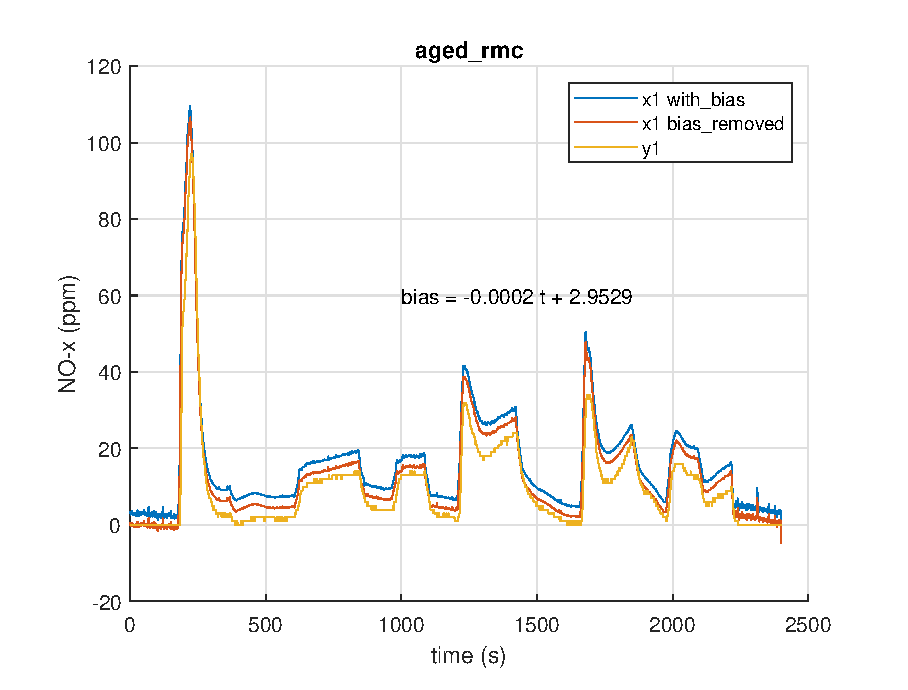
\includegraphics[width=\textwidth]{./figs/2-data/chi_est/aged_rmc_NOx_bias.eps}
        \end{figure}
    \end{minipage}
    \begin{minipage}{0.49\textwidth}
        \begin{figure}[H]
            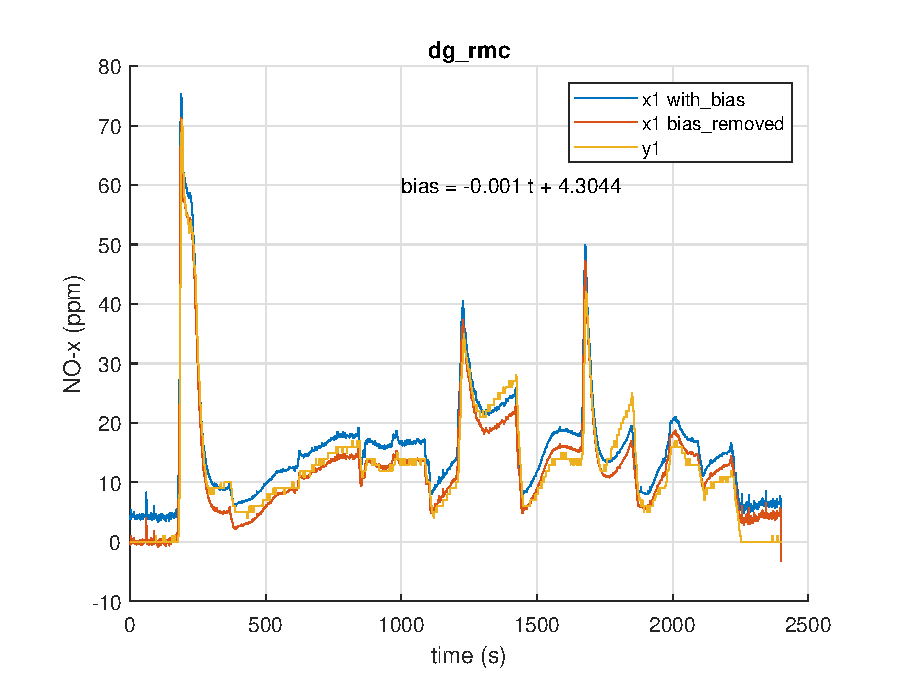
\includegraphics[width=\textwidth]{./figs/2-data/chi_est/dg_rmc_NOx_bias.eps}
        \end{figure}
    \end{minipage}
        \caption{Sensor bias correction for RMC cycles}
        \label{fig::bias_corr}
\end{figure}
The results depicted in Figure~\ref{fig::bias_corr} indicate that the coefficient of \( t \), \( b_1 \) (drift), is
considerably smaller in comparison to the bias \( b_0 \), suggesting it can be disregarded.

\subsubsection{Effect of $NH_3$ sensor bias and minimum threshold for cross-sensitivity}
The ammonia sensor used for ammonia measurement also has bias and there is a threshold on ammonia for which the $NO_x$
sensor becomes cross-sensitive to ammonia. Thus the expression for cross-sensitivity becomes:
\begin{align*}
    y_1 &= \lr{x_1 - b_0} + \chi (x_2 - b_{th})\\
\end{align*}

\subsubsection{Least-squares estimation assuming temperature independence}
The temperature changes in the RMC cycle do not affect the cross-sensitivity factor significantly. Thus, it can be treated as
a constant with respect to temperature fluctuations in that range. We have,
\begin{align*}
    \underbrace{y_1 - x_1}_{\pmb y} &= \underbrace{\bm{x_2 & -1}}_{\pmb \phi^T} \underbrace{\bm{ \chi \\ \underbrace{\chi b_{th} + b_0}_{=b}}}_{ \pmb \theta}\\
\end{align*}
Using the above model, the least-squares estimation of $\chi$ and $b$ is performed for RMC cycles. The results are shown
in Figure~\ref{fig::chi_est} and the error in estimation is shown in Figure~\ref{fig::chi_error}.
\begin{figure}[!ht]
    \begin{minipage}{0.49\textwidth}
        \begin{figure}[H]
            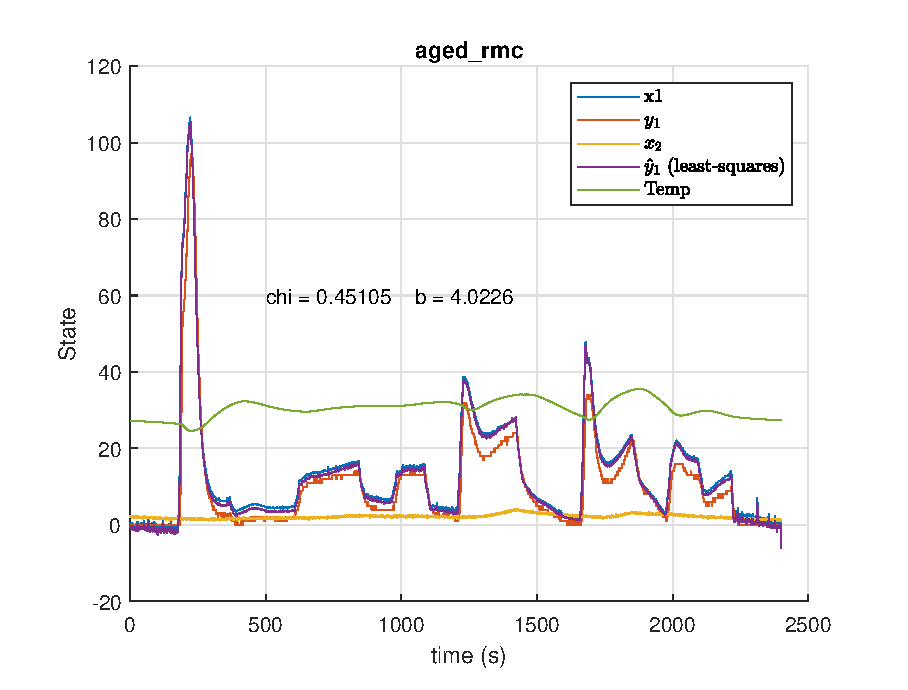
\includegraphics[width=\textwidth]{./figs/2-data/chi_est/aged_rmc_chi.eps}
        \end{figure}
    \end{minipage}
    \begin{minipage}{0.49\textwidth}
        \begin{figure}[H]
            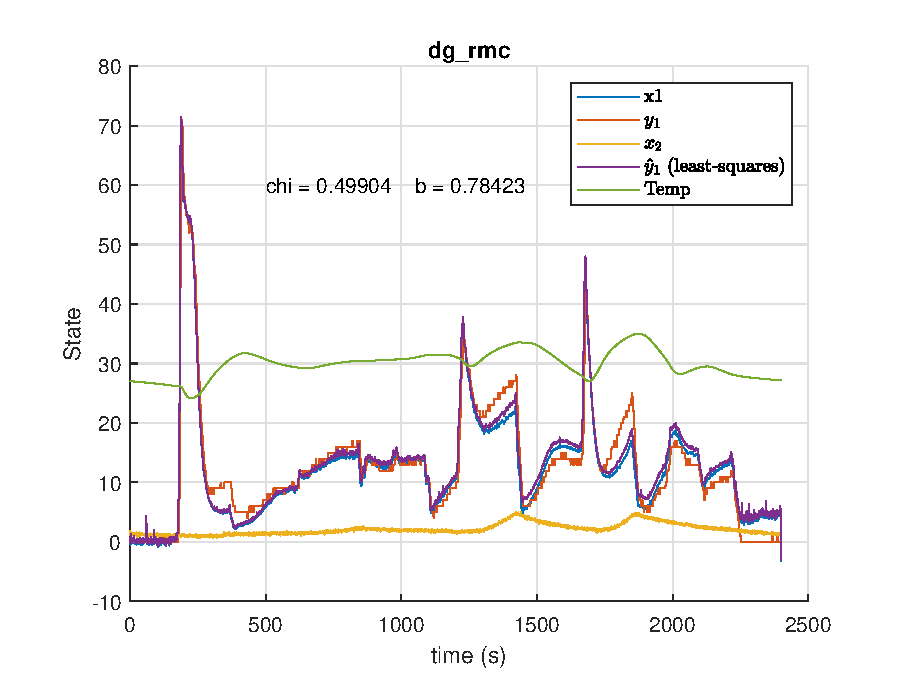
\includegraphics[width=\textwidth]{./figs/2-data/chi_est/dg_rmc_chi.eps}
        \end{figure}
    \end{minipage}
        \caption{$\chi$ estimation for RMC cycles}
        \label{fig::chi_est}
\end{figure}
\begin{figure}[!ht]
    \centering
    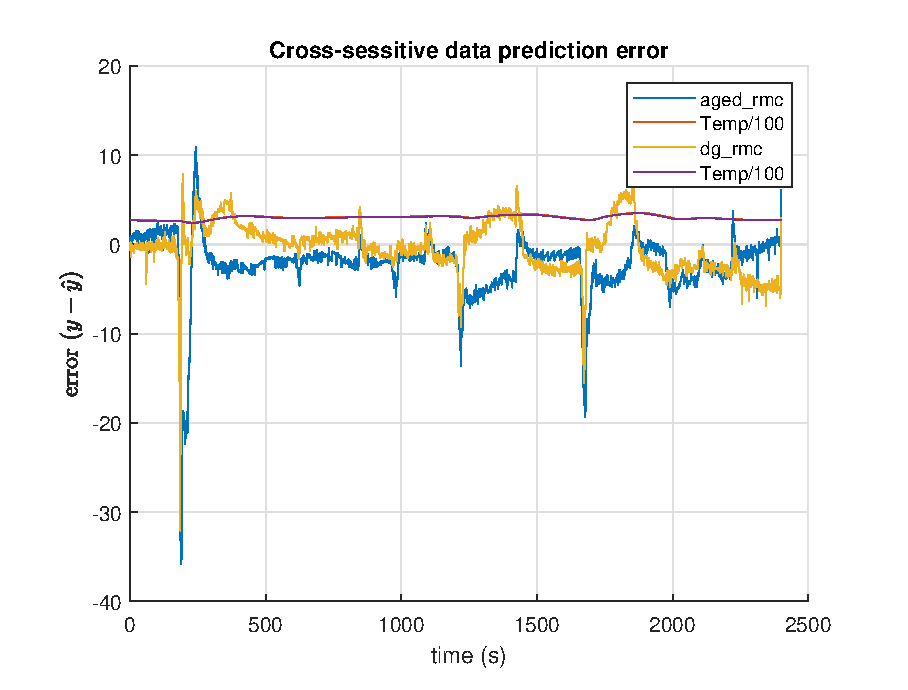
\includegraphics[width = 0.5 \textwidth]{./figs/2-data/chi_est/chi_error.eps}
    \caption{Error in $\chi$ estimation}
    \label{fig::chi_error}
\end{figure}
The error can be reduced by introducing the effects of temperature into $\chi$.

\subsubsection{Least-squares estimation with $\chi$ as a temperature function}
For simplicity, $\chi$ is assumed to be a linear function of temperature.
\begin{align*}
    \chi(T) &= a T - b_T
\end{align*}
Assuming the sensor-bias is not time-varying ($\because$ $b_1$ is small). The sensor bias, cross-sensitivity threshold
and temperature dependence can be combined into:
\begin{align*}
    y_1 &=  \lr{x_1 - b_0} + \lr{aT - b_{T}} \lr{x_2 - b_{th}}\\
    \lr{y_1 - x_1} &= a T x_2 - a b_{th} T - b_{T} x_2 + (b_T b_{th} - b_0)\\
    \underbrace{y_1 - x_1}_{\pmb y} &= \underbrace{\bm{T x_2 & -T & -x_2 & 1}}_{\pmb \phi^T} \underbrace{\bm{a \\ a b_{th} \\ b_T \\ b_T b_{th} - b_0}}_{\pmb \theta}\\
\end{align*}
The least-squares estimation of the parameters is performed using the above model and the results are shown in Figure~\ref{fig::chi_est_T} and the error in estimation is shown in Figure~\ref{fig::chi_error_comp}.
\begin{figure}[!ht]
    \begin{minipage}{0.49\textwidth}
        \begin{figure}[H]
            \includegraphics[width=\textwidth]{./figs/2-data/chi_est/aged_rmc_chiT.eps}
        \end{figure}
    \end{minipage}
    \begin{minipage}{0.49\textwidth}
        \begin{figure}[H]
            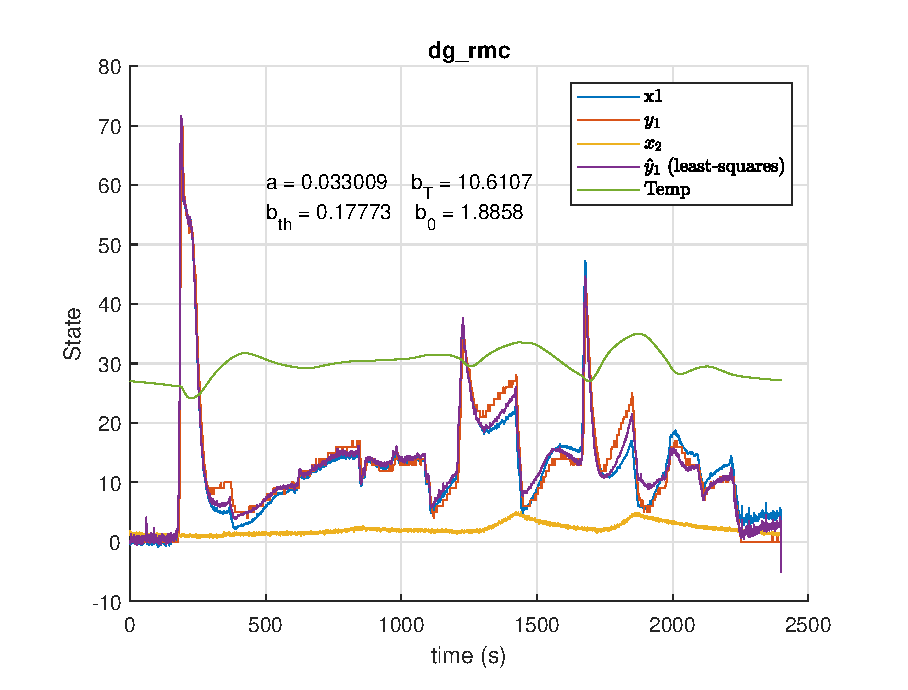
\includegraphics[width=\textwidth]{./figs/2-data/chi_est/dg_rmc_chiT.eps}
        \end{figure}
    \end{minipage}
        \caption{$\chi$ estimation for RMC cycles}
        \label{fig::chi_est_T}
\end{figure}
\begin{figure}[!ht]
    \begin{minipage}{0.49\textwidth}
        \begin{figure}[H]
            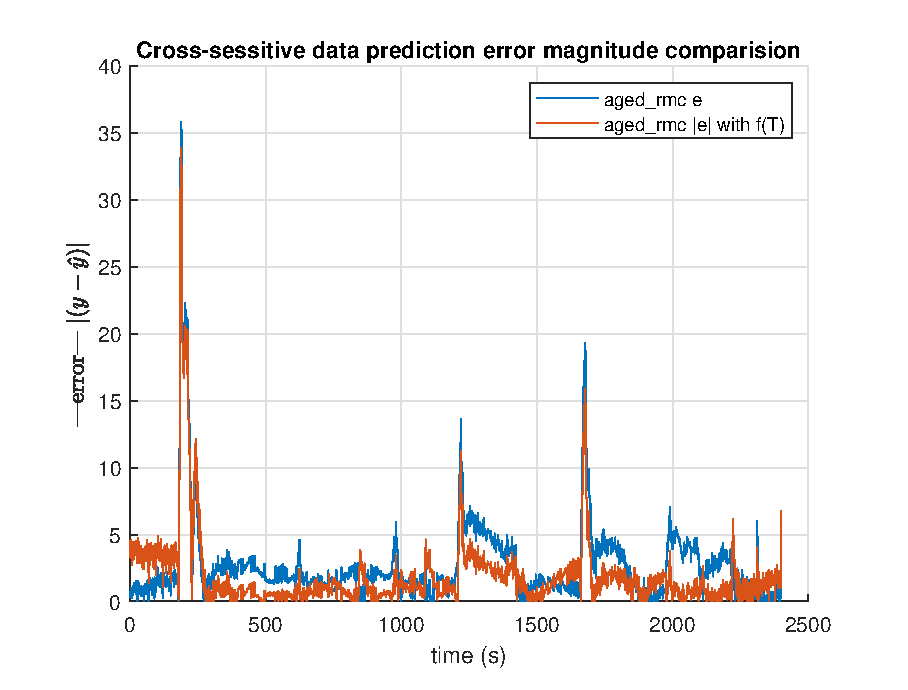
\includegraphics[width=\textwidth]{./figs/2-data/chi_est/aged_error_comp.eps}
        \end{figure}
    \end{minipage}
    \begin{minipage}{0.49\textwidth}
        \begin{figure}[H]
            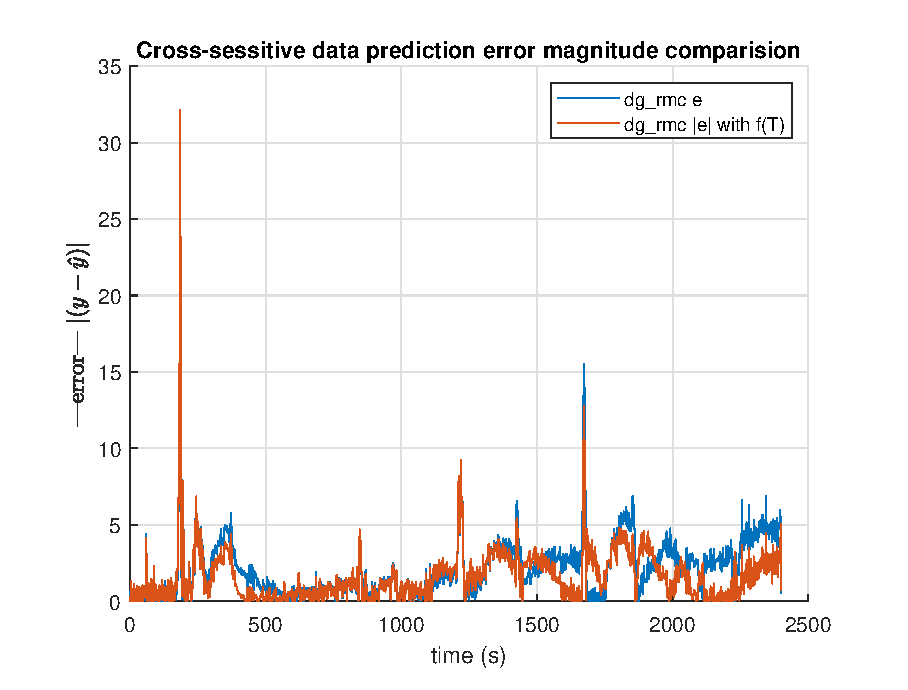
\includegraphics[width=\textwidth]{./figs/2-data/chi_est/dg_error_comp.eps}
        \end{figure}
    \end{minipage}
        \caption{Effect of temperature on prediction errors for $\chi$ estimation in RMC cycles}
        \label{fig::chi_error_comp}
\end{figure}
Introducing temperature clearly decreases the prediction error (Figure~\ref{fig::chi_error_comp}) in the model. However,
the reduction in error, while noticeable, is not significant when compared to the temperature-independent model
(Figure~\ref{fig::chi_error}), whose error remains within acceptable limits. Moreover, tailpipe ammonia measurements are
required for estimation of the cross-sensitivity error. Hence, for the current work, the cross-sensitivity effect is
treated as an unknown bounded disturbance.

% =============================================================================





\section{Data Preprocessing in Test-Cell and Truck Data}



\section{Test-Cell Data Preprocessing}
% \subsection{Test Data Signal Ranges}
The ranges of the measurement signals are tabulated bellow:
\begin{table}[H]
\centering
\begin{tabular}{c c c c c}
\hline \hline
Variable & Units & & & \\
\hline \hline
Degreend Data & & Cold FTP & Hot FTP & RMC\\ \hline
$T$   & $+200 \, ^0C$ & [60.96, -174.0] & [67.38, -64.7] & [148.76, 43.76]
\\
$F$   & $g/s$ & [439.04, 0.0]& [431.14, 0.0]& [403.84, 32.65]
\\
$x_1$ & $mol/m^3$ & [17.24, -2.97] &  [3.55, -0.57]& [2.23, 0.14]
\\
$x_2$ & $mol/m^3$ & [0.06, 0.0] & [0.17, -0.01] & [0.27, 0.06]
\\
$u_1$ & $mol/m^3$ & [20.16, 0.0] & [16.46, 0.0] & [24.26, 0.0]
\\
$u_2$ & $mol/m^3$ & [1.4, 0.0] & [1.0, 0.0] & [0.71, 0.01]
\\
$y_1$ & $mol/m^3$ & [0.07, 0.0]& [0.82, 0.0]& [2.11, 0.0]
\\
\hline
Aged Data & &Cold FTP & Hot FTP & RMC\\ \hline
$T$   & $+200 \, ^0C$ & [67.03, -172.85]& [72.5, -56.35]& [154.38, 48.18]
\\
$F$   & $g/s$ & [416.85, 0.0]& [418.24, 0.0]& [409.59, 32.63]
\\
$x_1$ & $mol/m^3$ & [25.03, 0.01] & [4.9, -0.42] & [3.24, 0.08]
\\
$x_2$ & $mol/m^3$ & [0.04, 0.0] & [0.6, -0.02] & [0.23, 0.08]
\\
$u_1$ & $mol/m^3$ &  [18.58, 0.0]& [16.26, 0.0] & [22.89, 0.0]
\\
$u_2$ & $mol/m^3$ & [1.31, 0.0] & [1.0, 0.0] & [0.67, 0.01]
\\
$y_1$ & $mol/m^3$ & [0.09, 0.0]& [1.06, 0.0]& [2.86, 0.0]
\\
\hline \hline
\end{tabular}
\caption{Test cell data ranges}
\end{table}


%==============================================================================

% \subsection{Signal Processing Steps}
The signal processing steps for getting the viable data used for model validation are summarized bellow.
\begin{figure}[H]
        \centering
        \includegraphics[width = 0.9\textwidth]{./figs/2-data/DataProcessingPipeline.png}
        \caption{Summary of Signal Processing Steps for Test Cell Data}
\end{figure}


% ==============================================================================

\section{Truck Data Preprocessing}
% \subsection{Truck Data Signal Ranges}
The ranges of the measurement signals are tabulated below:
\begin{table}[H]
\centering
\begin{tabular}{c c c c c c}
\hline \hline
Variable & Units & & & & \\
\hline \hline
Degreened Data & & adt\_15 & mes\_15 & wer\_15 & trw\_15 \\ \hline
$T$   & $+200 \, ^0C$ & [135.71, -79.68]& [116.91, -93.05]& [98.7, -142.85]& [125.21, -169.55]
\\
$F$   & $g/s$ & [425.94, 15.82]& [529.08, 0.0]& [386.51, 0.0]& [559.86, 0.0]
\\
$u_1$ & $mol/m^3$ & [27.34, 0.0]& [103.47, -6.87]& [49.99, 0.0]& [100.22, -6.73]
\\
$u_2$ & $mol/m^3$ & [0.89, 0.0]& [1.5, 0.0]& [1.07, 0.0]& [2.18, 0.0]
\\
$y_1$ & $mol/m^3$ & [24.66, 0.0] & [20.86, 0.0] & [22.51, 0.0]& [30.73, 0.0]
\\
\hline
Aged Data & & adt\_17 & mes\_18 & wer\_20 & trw\_16 \\ \hline
$T$   & $+200 \, ^0C$ & [111.04, -150.35]& [173.4, -86.67]& [353.84, -127.68]& [152.48, -155.45]
\\
$F$   & $g/s$ & [440.63, 0.0]& [391.06, 0.0]& [425.77, 0.0]& [569.7, 0.0]
\\
$u_1$ & $mol/m^3$ & [41.76, 0.0]& [36.89, 0.0]& [35.16, 0.0]& [68.93, 0.0]
\\
$u_2$ & $mol/m^3$ & [1.88, 0.0]& [1.07, 0.0]& [1.28, 0.0]& [1.66, 0.0]
\\
$y_1$ & $mol/m^3$ & [9.14, 0.0]& [19.6, 0.0]& [49.99, 0.0]& [38.39, 0.0]
\\
\hline \hline
\end{tabular}
\caption{Truck data ranges}
\end{table}


% =============================================================================

% \subsection{Signal Processing Steps}
The road data was collected from trucks operating in the United States  for two days separated by a few years
(Table~\ref{tab::truck_data_summary}) during which the catalyst has aged based on the existing performance measures. The
data contains measurements of $NO_x$ sensors before and after the catalyst, as well as other required variables
including flow rate, temperature and urea injection rate. The data preporcessing includes,
\begin{enumerate}
        \item removing the rows with missing values,
        \item removing the rows whose operating temperature range is beyond range of $200-300 \,^0C$,
        \item interpolating the missing data if the data breaks are smaller than a minute, and finally,
        \item smooting the data using non-causal chebyshev filter.
\end{enumerate}
The preprocessed data is than partitioned into drive segments with no breaks which correspond to a continuous driving
period from engine start to engine stop.
%===
